\documentclass{beamer}


\usepackage[french]{babel}

\usepackage[T1]{fontenc}

\usepackage[utf8]{inputenc}


\usetheme{Warsaw}
\title{Nouvelle heuristique pour VRP}
\author{Clément Legrand}
\date{28 février 2018} 

\begin{document}

\section{Présentation heuristique}

\begin{frame}[plain]
\titlepage
\end{frame}

\begin{frame}{Description}
\underline{Intérêt}: heuristique simple à mettre en place, et performante.

\begin{block}{Etapes de l'algorithme:}
\begin{itemize}
\item Recherche solution initiale: Algorithme Clarke and Wright

\item Recherche de la "pire" arête

\item Optimisations locales ensuite par 3 opérateurs
\end{itemize}
\end{block}

\end{frame}

\section{Obtention de la pire arête}

\subsection{Caractériser une arête}

\begin{frame}{Comment caractériser une arête ?}
\begin{block}{Idée}
Trouver des liens entre les solutions (quasi-) optimales
\end{block}

Entraînement d'un modèle prédictif pour distinguer
les arêtes optimales des autres en s'aidant de caractéristiques:
\begin{itemize}
\item Largeur de la tournée
\item Profondeur de la tournée
\item Coût de la tournée
\end{itemize}

	\centering
	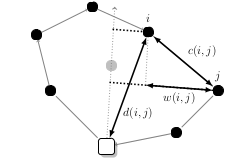
\includegraphics[height=0.4\textheight]{metrics.png}
	
\end{frame}

\subsection{Déterminer la pire arête}

\begin{frame}{Déterminer la pire arête}
Description spatiale précise d'une arête avec ces caractéristiques. 
\begin{center}
$b(i,j) = \frac{[\lambda_w w(i,j) + \lambda_c c(i,j)] [\frac{d(i,j)}{max_{k,l}d(k,l)}] ^ {\frac{\lambda_d}{2}}}{1+p(i,j)}$
\end{center}

\begin{itemize}
\item $p$ représente le nombre de fois où l'arête a été pénalisée (initialement 0)

\item Les paramètres $\lambda_w$,$\lambda_c$ et $\lambda_d$ valent $0$ ou $1$, et sont choisis selon le type d'instance.
\end{itemize}

\begin{exampleblock}{Pire arête}
La pire arête est celle qui maximise la fonction $b$.
\end{exampleblock}
\end{frame}

\section{Opérateurs locaux}

\subsection{Cross\_exchange}
\begin{frame}
Agit sur un couple de tournées, et essaie d'échanger toutes paires de séquence de clients consécutifs entre les deux routes. Complexité en $O(n^4)$: beaucoup trop...

\underline{Réduction}: si on connaît une arête à éliminer, on choisit la tournée correspondante. Et on ne s'intéresse qu'aux tournées qui ont des n\oe uds dans le voisinage de l'arête.

Complexité en théorie quadratique, mais proche de linéaire en général (beaucoup de solutions violent les contraintes)

	\centering
	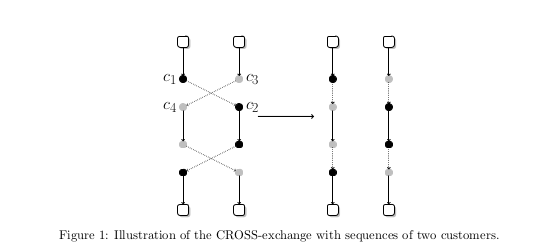
\includegraphics[height=0.4\textheight]{cross_exchange.png}
\end{frame}

\subsection{Ejection\_chain}
\begin{frame}
Agit (potentiellement) sur toutes les tournées. Commence par déplacer un client de la route $a$ vers la route $b$, de même en partant de $b$ vers $c$, jusque $l$ déplacements. 

	\centering
	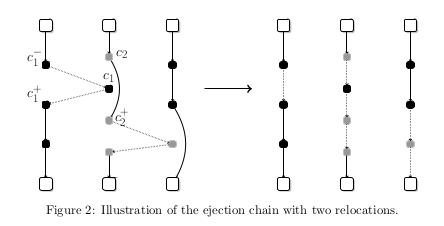
\includegraphics[height=0.4\textheight]{ejection_chain.png}
\end{frame}


\subsection{Lin-Kernighan Heuristic}
\begin{frame}

\begin{block}{Utilisation}
\begin{itemize}
\item Utilisé en général pour TSP;
\item Optimisation intra-tournée (chaque tournée est améliorée indépendamment des autres).
\end{itemize}
\end{block}

\begin{exampleblock}{Implémentation}
\begin{itemize}
\item Exécute i-opt (échange l'ordre de $i$ clients sur la tournée).
\item Si $i=k$ ou plus d'améliorations possibles $\rightarrow$ réalise la meilleure i-opt; recommence avec $i=2$
\item Si amélioration possible $\rightarrow$ recommence avec $i+1$
\item Si $i=2$ et pas d'améliorations possibles $\rightarrow$ on sort de la boucle.
\end{itemize}
\end{exampleblock}

\end{frame} 

\begin{frame}
\begin{alertblock}{Complexité}
Complexité en $O(n^k)$, $k$ choisi par l'utilisateur. En général exécution sur des morceaux de tournée.
\end{alertblock}

\begin{center}

\end{center}

\end{frame}


\section{Améliorations}
\begin{frame}
Si on ne trouve plus d'améliorations
\begin{itemize}
\item Optimisation globale (application des opérateurs sur l'ensemble du graphe): très coûteux
\item Remise à zéro des pénalités
\item Changement de la fonction de pénalisation

\end{itemize}

\end{frame}

















\end{document}